\documentclass[11pt, a4paper]{article}

\usepackage{tikz}
\usetikzlibrary{shapes.geometric, arrows.meta, positioning, calc}
\usepackage{amsmath, amssymb, bm}
\usepackage[margin=1in]{geometry}
\pagestyle{empty}

\definecolor{ucbblue}{RGB}{0, 51, 102}

\begin{document}

\begin{center}
    \textbf{\Large Mismo Eje Físico, Distinta Representación Coordenada[cite: 10]}
    \vspace{1cm}
    
    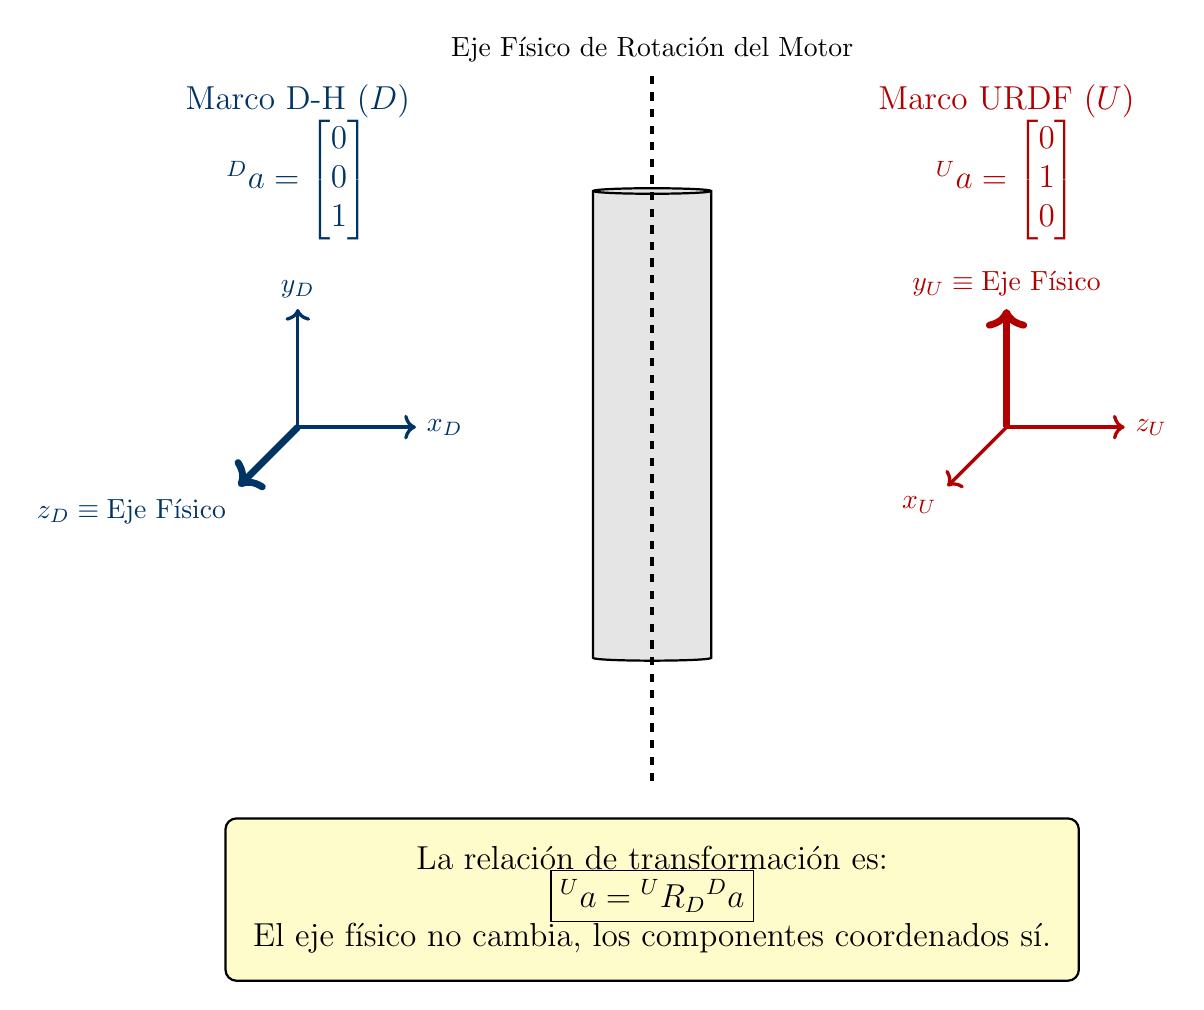
\begin{tikzpicture}[scale=1.5, thick]
        % Physical axis (Cylinder)
        \node[cylinder, draw=black, aspect=0.3, minimum height=6cm, minimum width=1.5cm, shape border rotate=90, fill=gray!20] (cyl) at (0,0) {};
        \draw[dashed, line width=1.5pt] (0,-3) -- (0,3) node[above]{Eje Físico de Rotación del Motor};
        
        % D-H Frame (Left Side)
        \coordinate (D) at (-3,0);
        \draw[->, ucbblue, line width=1.2pt] (D) -- ($(D)+(1,0)$) node[right]{$x_D$};
        \draw[->, ucbblue, line width=1.2pt] (D) -- ($(D)+(0,1)$) node[above]{$y_D$};
        \draw[->, ucbblue, line width=2.5pt] (D) -- ($(D)+(-0.5,-0.5)$) node[below left]{$z_D \equiv \text{Eje Físico}$};
        
        \node[above, ucbblue, font=\large, align=center] at (-3, 1.5) {Marco D-H ($D$) \\ ${}^{D}a = \begin{bmatrix} 0 \\ 0 \\ 1 \end{bmatrix}$};
        
        % URDF Joint Frame (Right Side - arbitrarily rotated)
        \coordinate (U) at (3,0);
        \draw[->, red!70!black, line width=1.2pt] (U) -- ($(U)+(1,0)$) node[right]{$z_U$};
        \draw[->, red!70!black, line width=2.5pt] (U) -- ($(U)+(0,1)$) node[above]{$y_U \equiv \text{Eje Físico}$};
        \draw[->, red!70!black, line width=1.2pt] (U) -- ($(U)+(-0.5,-0.5)$) node[below left]{$x_U$};
        
        \node[above, red!70!black, font=\large, align=center] at (3, 1.5) {Marco URDF ($U$) \\ ${}^{U}a = \begin{bmatrix} 0 \\ 1 \\ 0 \end{bmatrix}$};
        
        % Relationship Equation
        \node[fill=yellow!20, draw=black, rounded corners, inner sep=10pt, align=center, font=\large] at (0, -4) {
            La relación de transformación es: \\
            $\boxed{{}^{U}a = {}^{U}R_D {}^{D}a}$ \\
            El eje físico no cambia, los componentes coordenados sí.
        };
    \end{tikzpicture}
\end{center}

\end{document}
